\chapter{Электронно-цифровая подпись} \label{chapt4}%
\textbf{Мета роботи:~}%
Принцип работы, особенности, создание и использование ЭЦП.
\section{Теоретические ведомости} \label{sect4_a}
% https://www.youtube.com/watch?v=nrW_v8OBOno
% https://habrahabr.ru/post/194664/
% https://tools.ietf.org/html/rfc5280

В современном мире происходит постепенная замена бумажной технологии
обработки информации её электронным аналогом. Всё большее распространение
получают автоматизированные системы обработки информации. Тенденция ведет в
будущем к полной замене бумажного докуменоборота электронным. Однако защитных
атрибутов бумажных документов, таких как подписей, печатей, водяных знаков и
специальной фактуры поверхности,  - у электронного представления документа
нет. Поэтому возникла задача разработки такого механизма электронной защиты,
который смог бы заменить подпись и печать на бумажных документах. Во-первых,
такой механизм должен подтверждать, что подписывающее лицо не случайно
подписало электронный документ. Во-вторых, он должен подтверждать, что только
подписывающее лицо, и только оно, подписало электронный документ. В-третьих,
он должен зависеть от содержания подписываемого документа и времени его
подписания. В-четвертых, подписывающее лицо не должно иметь возможности в
последствии отказаться от факта подписи документа. Таким механизмом стала
электронно-цифровая подпись.

\textbf{Электронная цифровая подпись (ЭЦП)} --- реквизит электронного
документа, предназначенный для защиты данного электронного документа от
подделки, полученный в результате криптографического преобразования
информации с использованием закрытого ключа электронной цифровой подписи и
позволяющий идентифицировать владельца сертификата ключа подписи, а также
установить отсутствие искажения информации в электронном документе
(Федеральный Закон «Об электронно-цифровой подписи»).

\textbf{Криптографическое преобразование } --- это преобразование информации,
основанное на некотором алгоритме, зависящем от изменяемого параметра (обычно
называемого секретным ключом), и обладающее свойством невозможности
восстановления исходной информации по преобразованной, без знания
действующего ключа, с трудоемкостью меньше заранее заданной.Другими словами,
ЭЦП - это часть электронного документа, а фактически - обычный файл,
полученный в результате криптографического преобразования  документа.
Электронная подпись создаётся при помощи так называемого закрытого ключа.
Проверяется же отправленный документ открытым ключом - он общедоступен и
вместе с документом приходит получателю. То есть, ЭЦП использует т.н.
асимметричное криптографическое преобразование, в котором используется пара
ключей - открытый (публичный) ключ и секретный (личный, индивидуальный) ключ,
известный только одной взаимодействующей стороне. При использовании ЭЦП
гарантируется следующее. Во-первых, то, что документ не изменился в процессе
пересылки. Если после подписания цифровой подписью документ был искажен, это
выяснится при проверке открытым ключом. Во-вторых - гарантируется однозначная
идентификация отправителя. В случае с обычной подписью это можно сделать,
например, сравнив с подписью в паспорте. В случае с ЭЦП - специальные
удостоверяющие центры, выдающие сертификаты ключей.

\textbf{Закрытый ключ электронной цифровой подписи} --- уникальная
последовательность символов, известная владельцу сертификата ключа подписи и
предназначенная для создания в электронных документах электронной цифровой
подписи с использованием средств электронной  подписи;

\textbf{Открытый ключ электронной цифровой подписи} --- уникальная
последовательность символов, соответствующая закрытому ключу электронной
цифровой подписи, доступная любому пользователю информационной системы и
предназначенная для подтверждения с использованием средств электронной
цифровой подписи подлинности электронной цифровой подписи в электронном
документе;

\textbf{Сертификат ключа подписи} --- документ на бумажном носителе или
электронный документ с электронной цифровой подписью уполномоченного лица
удостоверяющего центра, которые включают в себя открытый ключ электронной
цифровой подписи и которые выдаются удостоверяющим центром участнику
информационной системы для подтверждения подлинности электронной цифровой
подписи и идентификации владельца сертификата ключа подписи;

\begin{figure}
  \centering
  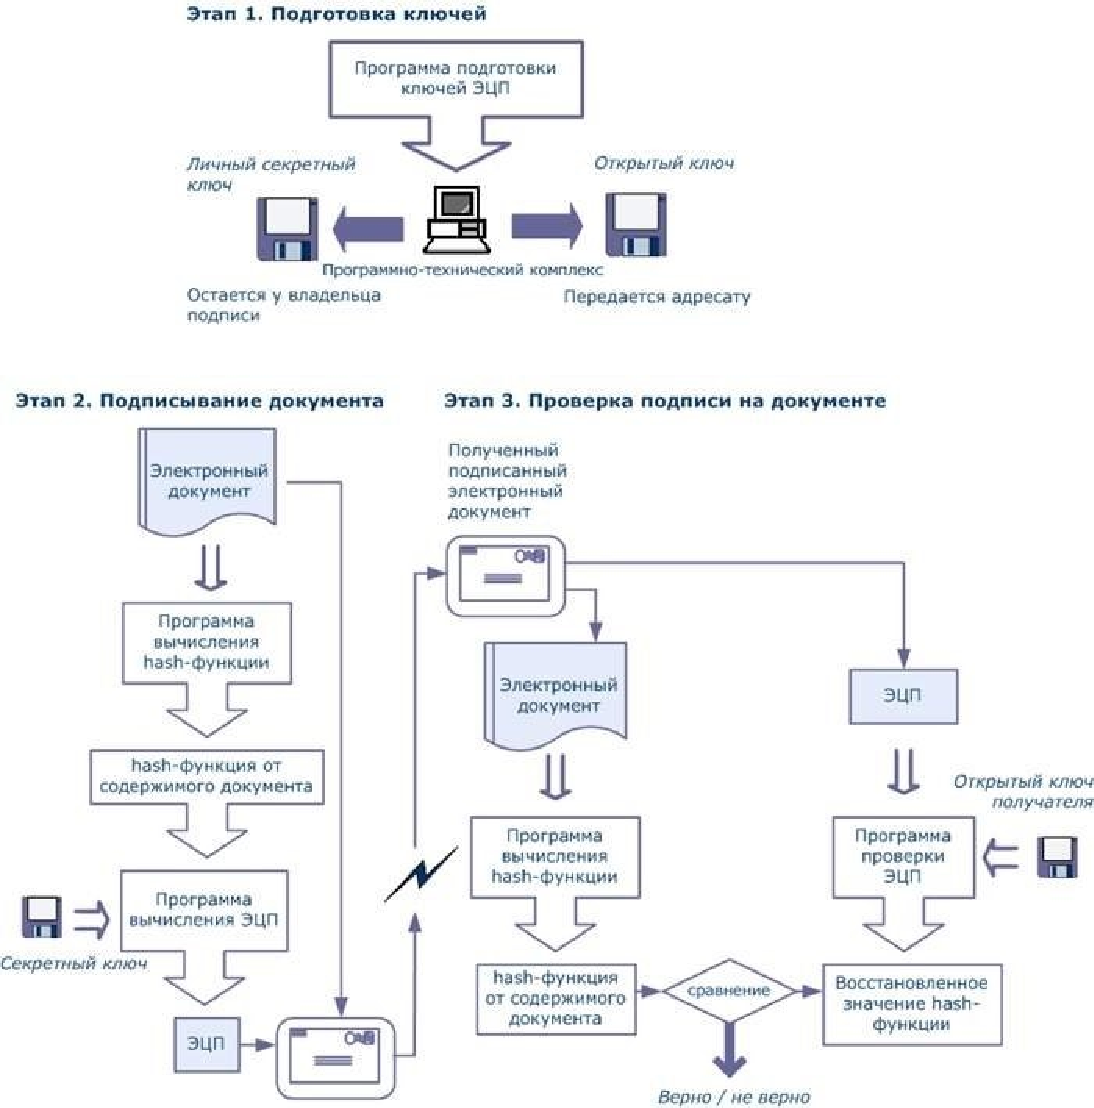
\includegraphics[width=\linewidth]{lab-4_1}
  \caption{Схема механизма ЭЦП, использующего асимметричное криптографическое преобразование}\label{img:4_1}
\end{figure}
При использовании асимметричного криптографического преобразования возникает
задача обеспечения совместного использования зашифрованной (подписанной)
информации, связанная с управлением ключами (генерация, распределение и
т.д.). Для решения этой трудоемкой задачи создаются специальные
удостоверяющие центры, услуги которых призваны облегчить использование ЭЦП.

\textbf{Удостоверяющий центр} --– это юридическое лицо, согласно Закону «Об
электронно-цифровой подписи» выполняющее следующие функции:

\begin{Notes}
\item изготовление сертификатов ключей подписей;
\item  создание (генерация) ключей
    электронных цифровых подписей по обращению клиентов  с гарантией
    сохранения в тайне закрытого ключа электронной цифровой подписи;
\item приостановка и возобновление действия сертификатов ключей подписей, а
    также их аннулирование;
\item ведение реестра сертификатов ключей подписей, обеспечение его
    актуальности и
возможности свободного доступа к нему клиентов;
\item  проверка уникальности открытых ключей электронных цифровых подписей в
    реестре сертификатов ключей подписей и архиве удостоверяющего центра;
\item выдача сертификатов ключей подписей в форме документов на бумажных
    носителях
и (или) в форме электронных документов с информацией об их действии;
\item осуществление по обращениям пользователей сертификатов ключей подписей
    подтверждение подлинности электронной цифровой подписи в электронном
    документе в отношении выданных им сертификатов ключей подписей;
\item предоставление клиентам иных связанных с использованием электронных
    цифровых подписей услуги.
\end{Notes}

\begin{figure}[ht]
  \centering
  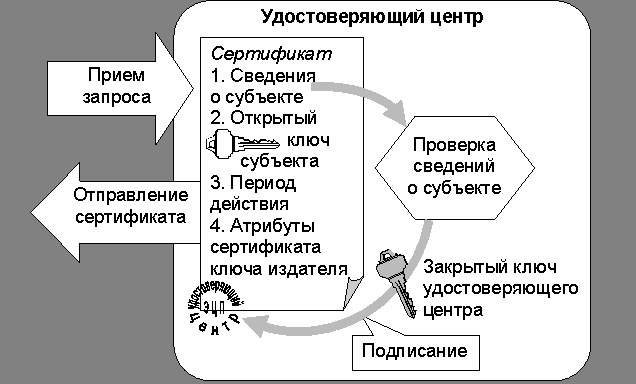
\includegraphics[width=\linewidth]{lab-4_2}
  \caption{Реализация механизма ЭЦП через Удостоверяющий центр }\label{img:lab4-2}
\end{figure}
Таким образом, задачу подтверждения ЭЦП, а также другие связанные задачи,
берет на себя удостоверяющий центр.

\textbf{Подтверждение подлинности электронной цифровой подписи в электронном
документе} --- положительный результат проверки соответствующим
сертифицированным средством электронной цифровой подписи с использованием
сертификата ключа подписи принадлежности электронной цифровой подписи в
электронном документе владельцу сертификата ключа подписи и отсутствия
искажений в подписанном данной электронной цифровой подписью электронном
документе.

\paragraph{Структура сертификата}
%http://rsdn.org/article/ASN/ASN.xml
Формат сертификата открытого ключа определен в рекомендациях Международного
Союза по телекоммуникациям ITU (X.509) и документе RFC 3280 Certificate \&
CRL Profile организации инженерной поддержки Интернета Internet Engineering
Task Force (IETF). IETF является открытым интернациональным сообществом
исследователей, разработчиков сетевых протоколов, операторов и
производителей, занимающихся проблемами развития сетей Интернет и
обеспечением непрерывного функционирования существующей инфраструктуры. В
настоящее время основным принятым форматом является формат версии 3,
позволяющий задавать дополнения, с помощью которых реализуется определенная
политика безопасности в системе. Несмотря на то, что документ RFC 3820
адресован Интернет-сообществу, формат сертификата открытого ключа
предоставляет гибкий механизм передачи разнообразной информации и применяется
в корпоративных PKI.

Сертификат открытого ключа подписи или шифрования представляет собой
структурированную двоичную запись в формате абстрактной синтаксической
нотации ASN.1. Сертификат содержит элементы данных, сопровождаемые цифровой
подписью издателя сертификата (см. рис. 6.1). В сертификате имеется десять
основных полей: шесть обязательных и четыре опциональных. Большая часть
информации, указываемой в сертификате, не является обязательной, а содержание
обязательных полей сертификата может варьироваться. К обязательным полям
относятся:

\begin{itemize}
  \item серийный номер сертификата Certificate Serial Number;
  \item идентификатор алгоритма подписи Signature Algorithm Identifier;
  \item имя издателя Issuer Name;
  \item период действия Validity (Not Before/After);
  \item открытый ключ субъекта Subject Public Key Information;
  \item имя субъекта сертификата Subject Name.
\end{itemize}

Под субъектом сертификата понимается сторона, которая контролирует секретный
ключ, соответствующий данному открытому ключу. Наличие необязательных полей
характерно для сертификатов версий 2 и 3, к необязательным полям сертификата
относятся номер версии, два уникальных идентификатора и дополнения. Структура
сертификата представлена на \todo{рис. ниже}

\begin{figure}[h]
  \centering
  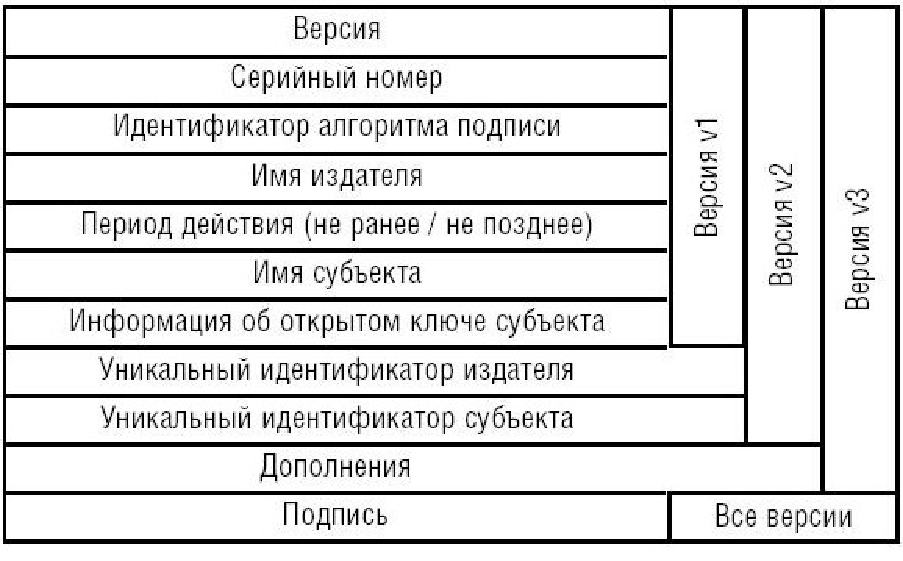
\includegraphics[width=\linewidth]{lab-4_3}
  \caption{Структура сертификата}\label{lab4_3}
\end{figure}

Издатель сертификатов присваивает каждому выпускаемому сертификату серийный
номер Certificate Serial Number, который должен быть уникален. Комбинация
имени издателя и серийного номера однозначно идентифицирует каждый
сертификат.

\subparagraph{\textmd{Поля} \texttt{Signature Аlgorithm Identifier}}
указывается идентификатор алгоритма ЭЦП, который использовался издателем
сертификата для подписи сертификата, например ГОСТ Р 34.10-94 \todo{(см. рис.
6.2)}.

\begin{figure}[h]
  \centering
  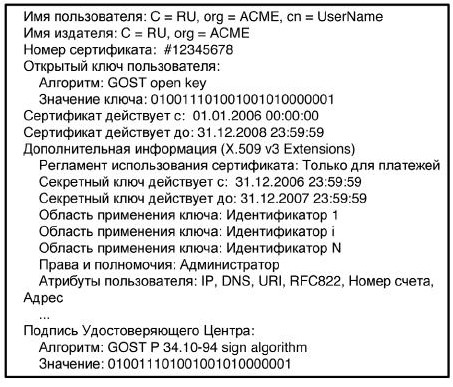
\includegraphics[width=\linewidth]{lab-4_4}
  \caption{Пример сертификата формата X.509}\label{lab4_4}
\end{figure}
 \subparagraph{\textmd{Поля} \texttt{Issuer Name}} содержит отличительное имя
(формата X.500) третьей доверенной стороны, то есть издателя, который
выпустил этот сертификат. В поле "Validity" (Not Before/After) указываются
даты начала и окончания периода действия сертификата.

\subparagraph{\textmd{Поля} \texttt{Subject Name}} содержит отличительное имя
субъекта, то есть владельца секретного ключа, соответствующего открытому
ключу данного сертификата. Субъектом сертификата может выступать УЦ, РЦ или
конечный субъект.

\subparagraph{\textmd{Поля} \texttt{Subject Public Key Information}} содержит
информацию об открытом ключе субъекта: сам открытый ключ, необязательные
параметры и идентификатор алгоритма генерации ключа. Это поле всегда должно
содержать значение. Открытый ключ и необязательные параметры алгоритма
используются для верификации цифровой подписи (если субъектом сертификата
является УЦ) или управления ключами.

\subparagraph{\textmd{Поля} \texttt{Issuer Unique Identifier} \textmd{и}
\texttt{Subject Unique Identifier}} Данные поля являются необязательными. Они
информируют об уникальных идентификаторах субъекта, издателя сертификата и
предназначены для управления многократным использованием имен субъектов и
издателей. Вследствие неэффективности подобного механизма управления
Интернет-стандарты профилей сертификата и списка аннулированных сертификатов
не рекомендуют использовать в сертификатах эти поля.

\subparagraph{Дополнения сертификата }

Важная информация находится также в дополнениях сертификата. Они позволяют
включать в сертификат информацию, которая отсутствует в основном содержании,
определять валидность сертификата и наличие у владельца сертификата прав
доступа к той или иной системе. Кроме того, в дополнениях содержится
технологическая информация, позволяющая легко проверить подлинность
сертификата. Каждая организация может использовать свои частные дополнения,
удовлетворяющие конкретным требованиям ведения бизнеса. Однако большинство
требований включено в стандартные дополнения, поддержку которых обеспечивают
коммерческие программные продукты.

Опциональное поле "Extensions" (дополнения) появляется в сертификатах третьей
версии. Каждое дополнение состоит из идентификатора типа дополнения Extension
identifier, признака критичности Criticality flag и собственно значения
дополнения Extension value. Идентификатор типа дополнения задает формат и
семантику значения дополнения. Признак критичности сообщает приложению,
использующему данный сертификат, существенна ли информация о назначении
сертификата и может ли приложение игнорировать данный тип дополнения. Если
дополнение задано как критичное, а приложение не распознает данный тип
дополнения, то сертификат не должен использоваться приложением. Приложение
может игнорировать нераспознанное некритичное дополнение и использовать
сертификат.

Дополнения сертификатов X.509 определены рекомендациями Х.509 версии 3
Международного Союза по телекоммуникациям и документом RFC 3280. Все эти
дополнения можно разделить на две категории: ограничивающие и информационные.
Первые ограничивают область применения ключа, определённого сертификатом, или
самого сертификата. Вторые содержат дополнительную информацию, которая может
быть использована в прикладном программном обеспечении пользователем
сертификата.

\noindent К ограничивающим дополнениям относятся:
\begin{enumerate}
  \item основные ограничения (Basic Constraints);
  \item назначение ключа (Key Usage);
  \item расширенное назначение ключа (Extended Key Usage);
  \item политики применения сертификата (Certificates Policies, Policy
      Mappings, Policy Constraints);
  \item ограничения на имена (Name Constraints).
\end{enumerate}

\noindent К информационным дополнениям относятся:
\begin{enumerate}
  \item идентификаторы ключей (Subject Key Identifier, Authority Key Identifier);
  \item альтернативные имена (Subject Alternative Name, Issuer Alternative Name);
  \item пункт распространения списка аннулированных сертификатов (CRL
      Distribution Point, Issuing Distribution Point);
  \item способ доступа к информации УЦ (Authority Access Info).

\end{enumerate}

\paragraph{Преимущества и недостатки ЭЦП}

Недостаток метода: хотя сообщение надежно шифруется, но <<засвечиваются>>
получатель и отправитель самим фактом пересылки шифрованного сообщения.

Общая идея криптографической системы с открытым ключом заключается в
использовании при зашифровке сообщения такой функции от открытого ключа и
сообщения (шифр -функции), которую алгоритмически очень трудно обратить, то
есть вычислить по значению функции её аргумент, даже зная значение ключа.

\subparagraph{Особенности системы }

Преимущество асимметричных шифров перед симметричными шифрами состоит в
отсутствии необходимости передачи секретного ключа. Сторона, желающая
принимать зашифрованные тексты, в соответствии с используемым алгоритмом
вырабатывает пару «открытый ключ -- закрытый ключ». Значения ключей связаны
между собой, однако вычисление одного значения из другого должно быть
невозможным с практической точки зрения. Открытый ключ публикуется в открытых
справочниках и используется для шифрования информации контрагентом. Закрытый
ключ держится в секрете и используется для расшифровывания сообщения,
переданного владельцу пары ключей. Начало асимметричным шифрам было положено
в 1976 году в работе Уитфилда Диффи и Мартина Хеллмана «Новые направления в
современной криптографии». Они предложили систему обмена общим секретным
ключом на основе проблемы дискретного логарифма. Вообще, в основу известных
асимметричных криптосистем кладётся одна из сложных математических проблем,
которая позволяет строить односторонние функции и функции-ловушки. Например,
криптосистема Ривеста-Шамира-Адельмана использует проблему факторизации
больших чисел, а криптосистемы Меркля-Хеллмана и Хора-Ривеста опираются на
так называемую задачу об укладке рюкзака.

\textbf{Недостатки} --- асимметричные криптосистемы требуют существенно
больших вычислительных ресурсов. Кроме того, необходимо обеспечить
аутентичность (подлинность) самих публичных ключей, для чего обычно
используют сертификаты.

\textbf{Гибридная (или комбинированная) криптосистема} --- это система
шифрования, обладающая всеми достоинствами криптосистемы с открытым ключом,
но лишенная её основного недостатка -- низкой скорости шифрования.

\emph{Принцип: }
Криптографические системы используют преимущества двух
основных криптосистем: симметричной и асимметричной криптографии. На этом
принципе построены такие программы, как PGP и GnuPG.

\subparagraph{Основной недостаток} асимметричной криптографии состоит в
низкой скорости из-за сложных вычислений, требуемых её алгоритмами, в то
время как симметричная криптография традиционно показывает блестящую скорость
работы. Однако симметричные криптосистемы имеет один существенный недостаток
-- её использование предполагает наличие защищённого канала для передачи
ключей. Для преодоления этого недостатка прибегают к асимметричным
криптосистемам, которые используют пару ключей: открытый и закрытый.

\emph{Шифрование: }Большинство шифровальных систем работают следующим
образом. Для симметричного алгоритма (3DES, IDEA, AES или любого другого)
генерируется случайный ключ. Такой ключ, как правило, имеет размер от 128 до
512 бит (в зависимости от алгоритма). Затем используется симметричный
алгоритм для шифрования сообщения. В случае блочного шифрования необходимо
использовать режим шифрования (например, CBC), что позволит шифровать
сообщение с длиной, превышающей длину блока. Что касается самого случайного
ключа, он должен быть зашифрован с помощью открытого ключа получателя
сообщения, и именно на этом этапе применяется криптосистема с открытым ключом
(RSA или Алгоритм Диффи -- Хеллмана). Поскольку случайный ключ короткий, его
шифрование занимает немного времени. Шифрование набора сообщений с помощью
асимметричного алгоритма -- это задача вычислительно более сложная, поэтому
здесь предпочтительнее использовать симметричное шифрование. Затем достаточно
отправить сообщение, зашифрованное симметричным алгоритмом, а также
соответствующий ключ в зашифрованном виде. Получатель сначала расшифровывает
ключ с помощью своего секретного ключа, а затем с помощью полученного ключа
получает и всё сообщение.

\subparagraph{Цифровая подпись обеспечивает}

\begin{Notes}
  \item Удостоверение источника документа. В зависимости от деталей определения
    документа могут быть подписаны такие поля, как «автор», «внесённые
    изменения», «метка времени» и т. д.
  \item Защиту от изменений документа. При любом случайном или преднамеренном
    изменении документа (или подписи) изменится шифр, следовательно, подпись
    станет недействительной.
  \item Невозможность отказа от авторства. Так как
    создать корректную подпись можно лишь, зная закрытый ключ, а он известен
    только владельцу, то владелец не может отказаться от своей подписи под
    документом.
\end{Notes}

\subparagraph{Возможные угрозы цифровой подписи}

\begin{Notes}
  \item Злоумышленник может попытаться подделать подпись для выбранного им документа.
  \item Злоумышленник может попытаться подобрать документ к данной подписи, чтобы подпись к нему подходила.
  \item Злоумышленник, укравший закрытый ключ, может подписать любой документ от имени владельца ключа.
  \item Злоумышленник может обманом заставить владельца подписать какой-либо документ, например используя протокол слепой подписи.
  \item Злоумышленник может подменить открытый ключ владельца на свой собственный, выдавая себя за него.
\end{Notes}

\textbf{Важной проблемой} всей криптографии с открытым ключом, в том числе и
систем ЭЦП, является управление открытыми ключами. Необходимо обеспечить
доступ любого пользователя к подлинному открытому ключу любого другого
пользователя, защитить эти ключи от подмены злоумышленником, а также
организовать отзыв ключа в случае его компрометации.

Задача защиты ключей от подмены решается с помощью сертификатов. Сертификат
позволяет удостоверить заключённые в нём данные о владельце и его открытый
ключ подписью какого-либо доверенного лица. В централизованных системах
сертификатов используются центры сертификации, поддерживаемые доверенными
организациями. В децентрализованных системах путём перекрёстного подписывания
сертификатов знакомых и доверенных людей каждым пользователем строится сеть
доверия.

Управлением ключами занимаются центры распространения сертификатов.
Обратившись к такому центру, пользователь может получить сертификат
какого-либо пользователя, а также проверить, не отозван ли ещё тот или иной
открытый ключ.

\paragraph{Применение ЭЦП}
Электронная цифровая подпись может быть использована в самых разнообразных
сферах деятельности. ЭЦП, как аналог собственноручной подписи, имеет целый
ряд преимуществ, обусловленных её электронной природой.

\begin{Notes}
  \item Юридически значимый электронный документооборот между субъектами хозяйственной деятельности. Электронный документооборот с использованием ЭЦП позволяет вести деловую переписку, а также заключать договора и обмениваться другими документами по электронной почте. При этом такие электронные документы будут иметь такую же юридическую силу, как и документы на бумаге, а невозможность подделки ЭЦП будет дополнительной гарантией вашего бизнеса.
  \item Эффективная обработка и хранение электронных документов. Электронный архив. Переход на электронный документооборот с использованием ЭЦП позволяет значительно повысить эффективность работы с документами в организации/предприятии. Электронными документами проще обмениваться, особенно в случае географически удаленной сети филиалов или представительств. Они занимают физически намного меньше места, что позволяет всегда иметь под рукой все необходимые документы. Использование функций шифрования позволяет гарантированно защитить документы от несанкционированного доступа не только во время передачи, но и при хранении в электронном архиве.
  \item Все это можно реализовать посредством специального программного обеспечения, которое поможет минимизировать проблемы при переходе на электронный документооборот и сделает работу с электронными документами интуитивно понятной и простой.
  \item Подача отчетности в электронном виде в государственные учреждения и организации. Применение ЭЦП позволяет значительно упростить и ускорить обмен документами между субъектами хозяйственной деятельности и контролирующими государственными структурами. Электронная форма подача отчетности подразумевает возможность обмена всеми необходимыми документами через Интернет, например с помощью электронной почты. При этом документы подписываются с помощью ЭЦП (что дает им юридическую силу) и шифруются (что позволяет защитить их от несанкционированного доступа). Подача отчетности в электронном виде позволяет сэкономить время, расходы на доставку и снизить риски связанные с человеческим фактором. К тому же проверка и обработка электронных документов может быть полностью автоматизирована, что минимизирует ошибки при проверке документа.
  \item Аутентификация и разграничение доступа. Технология ЭЦП имеет применение и в областях, не связанных с электронным документооборотом. Электронные ключи могут использоваться для получения доступа к управлению системами/механизмами требующими надежной аутентификации и протоколирования выполняемых операций.
\end{Notes}

\subparagraph{Текущие требования к стойкости ЭЦП}

\todo{пока пусто}

\paragraph{Проверка подлинности ЭЦП}
% http://nalog-nalog.ru/spravochnaya_informaciya/kak_proishodit_proverka_podlinnosti_ecp/
% http://referatwork.ru/category/tehnologii/view/475258_identifikaciya_i_proverka_podlinnosti

Одним из способов проверки подлинности ЭЦП является предоставление
сертификата, подтверждающего, что подпись и сертификат на момент подачи
документов актуальны и не утратили свою силу.

Сертификат ключа проверки электронной подписи может представлять собой как
электронный документ, так и удостоверение в бумажном виде, которые
подтверждают законное право владельца на электронную подпись и на ключ её
проверки.

Квалифицированные сертификаты ключа проверки подлинности электронной подписи
могут быть выданы лишь таким удостоверяющим центром, который обязательно
имеет аккредитацию или уполномочен на это федеральным органом.

\todo{Дополнить информацию для Украины}
\section{Задания}\label{sect4_b}

Уровень 1. %

\begin{enumerate}
  \item Выбрать и отобразить реестр сертификатов на Вашем устройстве.
  \item Опишите состав сертификата.
  \item Выберите шифрованный блок данных.
  \item Опишите полный путь данного сертификата к \todo{main-центру раздачи
      разрешений}.
\end{enumerate}

Уровень 2. %

\begin{enumerate}
  \item Создайте самоподписной сертификат.
  \item Внесите его в свой реестр.
  \item Приложите данные в отчёт.
\end{enumerate}

Уровень 3.%

\begin{enumerate}
  \item Напишите алгоритм для создания подписанного сертификата.
  \item Создайте сертификат подписанный ЭЦП из прошлого задания.
  \item Приложите пример работы программы и подписанный сертификат.
\end{enumerate}

\section{Пример выполнения работы}\label{sect4_c}
%
Пример будет включать создание ЭПЦ как самостоятельно, так и используя ПО.
\section{Варианты}\label{sect4_d}
%
\section{Вопросы для контроля}\label{sect4_e}
%
\begin{enumerate}
  \item Что такое электронно-цифровая подпись?
  \item Каков принцип работы ЭЦП?
  \item Почему ЭЦП используется в большинстве систем проверки документации?
  \item Опишите этапы шифрования-дешифровки.
  \item Как подпись обеспечивает целостность данных?
  \item Случаи небезопасного использования ЭПЦ?
  \item Где на компьютере могут храниться цифровые подписи?
  \item Как проверить надёжность ЭПЦ?
\end{enumerate}
